\chapter{Execute Stage}

\begin{wrapfigure}{l}{1.5in}
\caption{Execute}\label{fig:execute}
\begin{center}
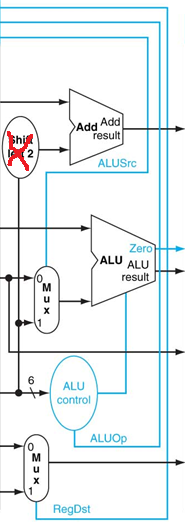
\includegraphics[width=1.5in]{../images/pipeline_execute.png}
\end{center}
\end{wrapfigure}

\WrapBarrier

Note that I put a red `x' over the left shift two unit.  In our case it is not needed, as we are a word addressable machine, so the address is correct as is.  The machine from the book is byte addressable, but word length for commands, thus the address must be multiplied by four (shifted left by two in binary) to handle this.  Our simpler machine helps us here.  Realize the left shift is easily handled by just appending two grounded wires on the right and dropping the two left most bits - a simple job for concatenation.  Though simple it is still something and since unneeded, it is left off.  The immediate value (from the sign extender) is passed directly to the adder.

\section{Assemble}

You have all the units you need to build the execute stage.  Make sure you follow the wiring in Fig~\ref{fig:execute} carefully.  Separate your signals into three categories: input, internal, output.  In this stage all output comes from the buffer, so the execute stage outputs must come from the buffer outputs.  I highlight the inputs, and wire them up first, marking each one complete with a red line when you do it.  Once that is done go through the internal wires.  There should be a wire for each already.  When you use a wire mark it with a red line to keep track.  You should finish quickly if you follow this methodology.

\subsection{Buffer}

The buffer is a simple design, just like the previous one and is provided to save time.  Adapt your prior testbench to verify.

\subsection{Mux and Adder}

Your mux and adder have been tested and used already so they do not require further testing.  Simply hook them up per Fig~\ref{fig:execute}. Validation will be done by testing the entire unit.

\subsection{ALU and Control}

You built and tested these last time, so this time you only need to instantiate.  Make sure you connect them as indicated in Fig~\ref{fig:execute}.

\section{Test}

Now you need to test it.  You should do a fake command of each type with data values that can test key functioning like overflow, etc.  Look at the command list and I would put each command as a comment in your testbench, followed by the settings to test it.  Do a couple data values for each, and it should be good.  Make sure you have a reason for your choices.

\section{Your Assignment}

You are to:
\begin{enumerate}
\item Write a testbench for the buffer, run a simulation and generate a timing diagram.
\item Integrate the units into execute and run your simulation and generate a timing diagram to verify it works.
\item  Write up a lab report in \LaTeX\ following the lab format in \verb1LabN.tex1 and generate a pdf file.
\item Upload the pdf and all the Verilog files to the course LMS.
\end{enumerate} 